We finally have all the main ingredients to generalize our line integral detour and discuss integration of $n$-forms over $n$-dimensional manifolds.

\section{Orientation}

\newthought{We know from calculus one}, or our line integral examples, that the direction in which we traverse the interval, or a curve, can actually make a difference.
Indeed, the sign of the integral of a differential $n$-form is only fixed after choosing an orientation of the manifold.

If for a curve an orientation is simply a choice of a direction along it, so we can make sense of it in terms of clockwise or counter-clockwise, generalising the concept will require an extra abstraction step.
Not just that, you have seen already that in $\R^n$ there is a standard orientation, but in other vector spaces we may need to make arbitrary choices.
For manifolds, the situation is much more complicated: for example, on a M\"obius strip\footnote{Cf. Example~\ref{ex:mobius}.} it is impossible to make any such choice, as it turns out, it is non-orientable.

Let's get there step by step.

\begin{definition}
  Let $V$ be a one-dimensional vector space. Then $V\setminus\{0\}$ has two components.
  An \emph{orientation} of $V$ is a choice of one of these components, which one then labels as ``positive'' and ``negative''.
  A \emph{positive basis} of $V$ then is a choice of any non-zero vector belonging to the positive component, while a \emph{negative basis} of $V$ is a choice of any non-zero vector belonging to the negative component.
\end{definition}

\begin{example}
  The standard orientation of $\R$ is give by declaring that the positive numbers are the positive components of $\R\setminus\{0\}$.
  A common choice as positive basis for $\R$ is $\{e_1 \equiv 1\}$ while a negative basis could be $\{-e_1\}$.
\end{example}

Let $V$ be a $n$-dimensional vector space.
How can we generalize in a meaningful way the definition above?

By Proposition~\eqref{prop:dimLkV}, the space $\Lambda^n(V)$ is a one-dimensional vector space.
Moreover, if $\{e_1,\ldots,e_n\}$ is a basis for $V$, then $e_1\wedge\cdots\wedge e_n$ is a basis for $\Lambda^n(V)$.

Looks like we are getting somewhere.

\begin{definition}
  Let $V$ be a $n$-dimensional vector space.
  An \emph{orientation} on $V$ is a choice of orientation on $\Lambda^n(V)$.
  \marginnote{It should be clear from this that the orientation is, in fact, an equivalence class of ordered bases.}
  Therefore there are exactly two orientations: we say that a basis $\{e_1,\ldots,e_n\}$ of $V$ is \emph{positive} (or positively oriented) if $e_1\wedge\cdots\wedge e_n$ is a positive basis of $\Lambda^n(V)$ and \emph{negative} (or negatively oriented) otherwise.
\end{definition}

\begin{example}
  If $e_i$ is the standard $i$th basis vector in $\R^n$, the standard orientation of $\R^n$ is given by declaring that $e_1\wedge\cdots e_n$ is a positive basis of $\Lambda^n(\R^n)$ and thus that $\{e_1,\ldots,e_n\}$ is a positive basis of $\R^n$.
\end{example}

The key in the preservation of orientation now resides only in the way different bases are transformed by $n$-forms, as the following lemma shows.

\begin{lemma}\label{lemma:orient}
  Let $V$ be a $n$-dimensional vector space and let $0\neq \omega\in\Lambda^n(V)$.
  Then, all bases $\{v_1, \ldots, v_n\}$ for which $\omega(v_1,\ldots v_n) > 0$ give the same orientation for $V$.
\end{lemma}
\begin{proof}
  Let $\{v_1, \ldots, v_n\}$ and $\{w_1, \ldots, w_n\}$ denote two different basis for $V$, then there exists a linear isomorphism $\varphi$ such that $v = \varphi w$, that is $v_i = \varphi_{i}^j w_j$.
  By definition and by multilinearity we then have
  \begin{equation}\label{eq:posorie}
    \omega(v_1,\ldots v_n) = \omega(\varphi w_1,\ldots \varphi w_n) = \det(\varphi)\omega(w_1,\ldots w_n) > 0,
  \end{equation} that is the positivity of $\omega$ on the bases characterize the set of bases.
\end{proof}

\begin{exercise}
  Let $V$ be a $n$-dimensional vector space, prove that two nonzero $n$-forms on $V$ determine the same orientation if and only if each is a positive multiple of the other.
\end{exercise}

\begin{remark}
  Of course, if $V$ is a vector space, then an orientation on $V$ canonically determines an orientation on the dual space $V^*$ by declaring that the basis dual to a positive basis is itself positive.
\end{remark}

We are almost there.
The tangent space is a vector space and $n$-forms act naturally on tangent vectors, this seems likely to be the right place to define an orientation for a manifold, at least pointwise.
As usual, one does need to make sure that all the local orientations just defined on the tangent bundle are gluing together coherently.

\begin{remark}
  If we look at a single chart $(U,\varphi)$, by Lemma~\ref{lemma:orient} each chart in the atlas determines an orientation at each point of its domain, which will be positive if $\det(D\varphi)>0$ and negative otherwise.
  This procedure can be repeated for each chart in an atlas for $M$.
  Thus, in order to get a globally consistent ordering, we need to worry about the overlaps between charts.
\end{remark}

\begin{definition}
  We call an atlas $\cA = \{(U_i,\varphi_i)\}$ \emph{oriented} if all the charts have the same orientation, that is, if $\det(D\varphi_{ij}) > 0$ for all the transition functions $\varphi_{ij} := \varphi_i\circ\varphi_j^{-1}$.

  A manifold $M$ with an oriented atlas is called \emph{oriented manifold}.
  If an orientation exists, we say tht $M$ is \emph{orientable}, in this case we call the equivalence class of atlases with the same orientation an \emph{orientation}.
  Otherwise we say that the manifold is \emph{nonorientable}.
\end{definition}

An immediate consequence of Lemma~\ref{lemma:orient} is that if a manifold is orientable, there are exactly two different orientations.

\begin{definition}
  Given an orientation on a manifold, we say that any chart from the same equivalence class of atlases is \emph{positively oriented}, while we call all other charts \emph{negatively oriented}.
\end{definition}

If $M$ is connected, as for vector spaces, an orientation on $\Lambda^n(M)$ determines the orientation of the manifold.
\marginnote{If it is not connected, then we need to deal with each connected component separately.}

\begin{theorem}
  Let $M$ be a $n$-dimensional smooth manifold.
  A nowhere-vanishing $n$-form $\omega\in\Omega^n(M)$ uniquely determines an orientation.
  For this reason, nowhere vanishing $n$-forms on a smooth $n$-manifold are called \emph{volume forms}.
\end{theorem}
\begin{proof}
  Let $\varphi$ and $\psi$ be two different charts with overlapping domains (otherwise there is nothing to check) and with local coordinates $(x^i)$ and $(y^i)$ respectively.
  Define the transition map $\varphi := \psi\circ\varphi^{-1}$, so that $(y^1,\ldots,y^n) = \varphi(x)$.
  Since $d y^j = (D\varphi)_i^j dx^i$, we have that locally
  \begin{align}
    \omega &= \widetilde \omega (y) dy^1\wedge\cdots\wedge dy^n \\
    &= (\widetilde\omega \circ \varphi)(x) \det(\varphi|_x) dx^{1}\wedge\cdots\wedge dx^{n} \\
    &= \omega(x) dx^{1}\wedge\cdots\wedge dx^{n},
  \end{align}
  where we used Proposition~\ref{prop:wedgeToJDet} and Theorem~\ref{thm:pullbacksdifferentialforms}.
  Thus, $\omega(x)$ and $\widetilde\omega(y)$ have the same sign if and only if $\det(D\varphi|_x) > 0$.
\end{proof}

\begin{definition}
  Let $M$ be a $n$-dimensional smooth manifold.
  If $(U,\varphi)$ is a chart with local coordinates $(x^i)$ such that, in the coordinate representation, $\omega = \omega(x) dx^1\wedge\cdots\wedge dx^n$ with $\omega(x) > 0$, then we say that the chart $\varphi$ is \emph{positively oriented} with respect to $\omega$, otherwise we say that it is \emph{negatively oriented}.  
\end{definition}

\begin{remark}
  In fact, this definition can be immediately extended to vector bundles.
  Given a real vector bundle $\pi: E \to M$, an orientation of $E$ means that for each fiber $E_p$, there is an orientation of the vector space $E_p$ such that each trivialization map
  \begin{equation}
    \varphi_{U}:\pi^{-1}(U)\to U\times \R^{n},
  \end{equation}
  with $\R^n$ equipped with its standard orientation, is fiberwise orientation-preserving.
  \marginnote[-2em]{Otherwise said, we can cover the manifold by (continuous) local frames whose local trivializations are orientation preserving.}

  With this definition, the orientability of $M$ coincides with the orientability of the bundle $M\to TM$.
\end{remark}

\begin{example}
  The euclidean space $\R^n$ is orientable with orientation given by the continuous global frame $\frac{\partial}{\partial r^i},\ldots,\frac{\partial}{\partial r^n}$.
\end{example}

\begin{example}\label{exe:orientsphere}
  Let $M = \bS^1\subset \R^2$.
  This is an orientable manifold and we can find an orientation using the stereographic projections from Exercise~\ref{ex:stereo}.
  Let $U_1 = \bS^1\setminus\{N\}$ and $U_2 = \bS^1\setminus\{S\}$, with the associated diffeomorphisms
  \begin{equation}
    \varphi_1(p) = \frac{2p^1}{1-p^2}
    \quad\mbox{and}\quad
    \varphi_2(p) = \frac{2p^1}{1+p^2}.
  \end{equation}
  Let's pick a pointwise orientation by choosing as basis $X_p\in T_pM$ given by $X_p = -p^2 \frac{\partial}{\partial p^1} + p^1 \frac{\partial}{\partial p^2}$.
  Then, on $U_1$,
  \begin{align}
    (\varphi_1)_*(X) &= (d\varphi_1)_p(X) \\
    &= \left(\begin{smallmatrix}
      \frac{2}{1-p^2} & \frac{2p^1}{(1-p^2)^2}
    \end{smallmatrix}\right)
    \left(\begin{smallmatrix}
      -p^2 \\ p^1
    \end{smallmatrix}\right) \frac{\partial}{\partial x}\Big|_{\varphi_1(p)}\\
    &= \frac{2}{1-p^2} \frac{\partial}{\partial x}\Big|_{\varphi_1(p)},
  \end{align}
  and $\frac{2}{1-p^2}>0$.
  If we perform the same computation on $U_2$, however, we obtain $(\varphi_2)_*(X) = -\frac{2}{1+p^2}\frac{\partial}{\partial x}\Big|_{\varphi_2(p)}$, with the negative coefficient $-\frac{2}{1+p^2} < 0$ (check!), corresponding to the opposite orientation on $U_2$.
  Of course, in this case, not all is lost: by choosing $\widetilde\varphi_2(p) = \varphi_2(-p^1, p^2)$ we obtain $(\widetilde\varphi_2)_*(X) = \frac{2}{1+p^2} \frac{\partial}{\partial x}\Big|_{\widetilde\varphi_2(p)}$ with the positive coefficient $\frac{2}{1+p^2} > 0$ (check!), which shows that $X_p$ defines an orientation on the whole $\bS^1$.
\end{example}

\begin{exercise}
  Check that the Jacobian determinant $\det(D(\varphi_2\circ \varphi_1^{-1}))$ of the transition chart from Exercise~\ref{exe:orientsphere} is negative, while $\det(D(\widetilde\varphi_2\circ \varphi_1^{-1}))$ is positive.
\end{exercise}

\begin{marginfigure}
  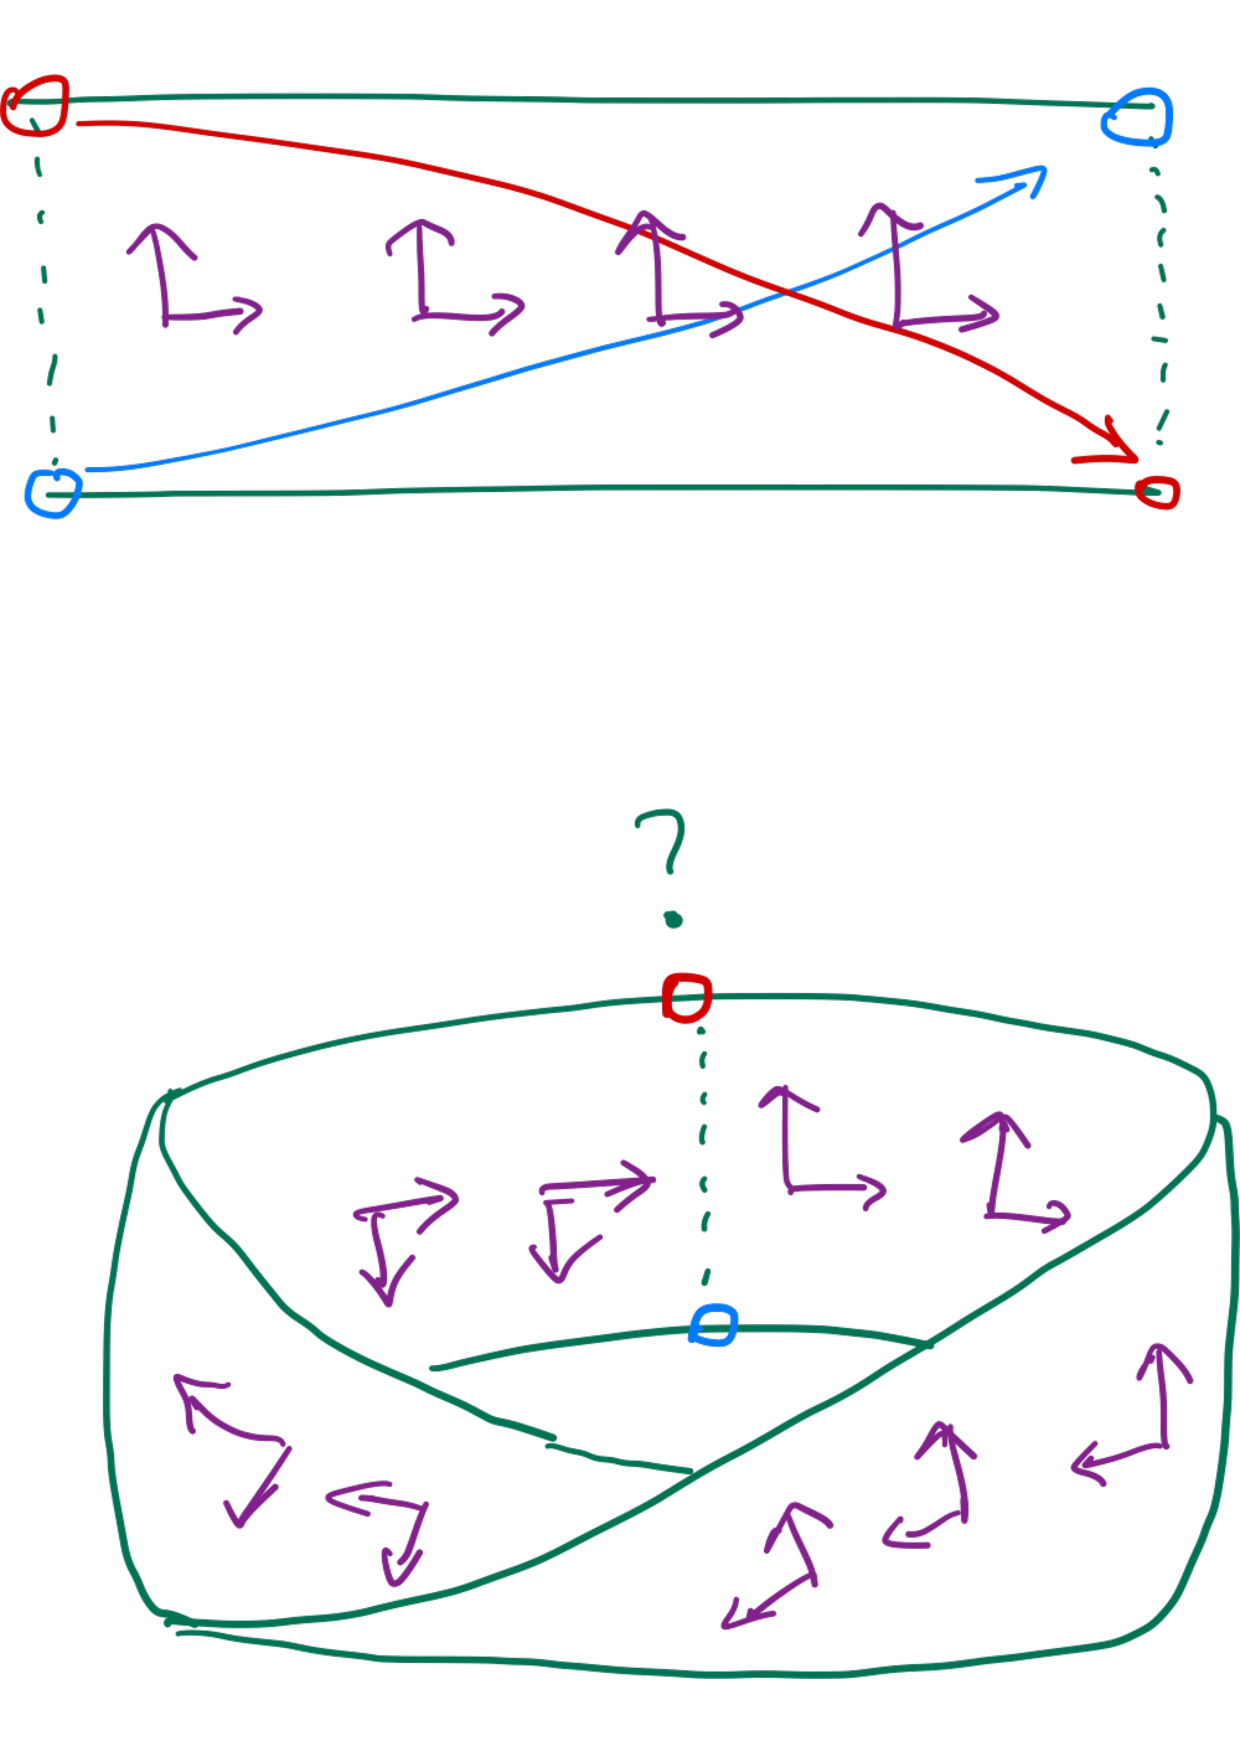
\includegraphics{7_1-mobius_strip.pdf}
\end{marginfigure}

\begin{exercise}
  Consider the open M\"obius strip $M$, a variation of Example~\ref{ex:mobius} defined as the quotient of $\R\times(-1,1)$ via the identification $(x,y) \sim (x+1, -y)$, and denote $\pi: \R\times(-1,1)\to M$ the corresponding projection map.
  The M\"obius strip inherits the differentiable structure from $\R^2$, so we need to show that there is no orientable atlas which is also compatible with the differentiable structure on $M$.
  \begin{enumerate}
    \item Define the map $\sigma:\R\times(-1,1)\to\R\times(-1,1)$ by $\sigma(x,y) = (x+1, -y)$ and show that $\pi\circ\sigma = \sigma$.
    \item If $\nu\in\Omega^2(M)$ define $f$ by $\pi^* \nu = f \omega$ where $\omega$ is an area\footnote{I.e. a volume $2$-form.} form on $\R\times(-1,1)$.
    Show that $f(x+1, y) = - f(x,y)$.
    \item Conclude that $f$ must vanish at some point of $\R\times(-1,1)$, which implies that $M$ is nonorientable.
  \end{enumerate}
\end{exercise}

What about orientation on the boundaries?

Let's first look at the tangent space. 

Let $M$ be a smooth $n$-manifold with boundary and $p\in \partial M$.
Then, we have three types of possible vectors:
\begin{enumerate}
  \item tangent boundary vectors: $X\in T_p(\partial M)\subset T_p M$ tangent to the boundary, forming an $(n-1)$-dimensional subspace of $T_p M$;
  \item inward pointing vectors: $X\in T_pM$ such that $X = \varphi^{-1}_*(Y)$ where $\varphi^{-1}: V\subset \cH^n \to M$ and $Y$ is some vector $Y = (Y^1, \ldots, Y_n)$ with $Y_n > 0$;
  \item outward pointing vectors: $X\in T_pM$ such that $-X$ is inward pointing.
\end{enumerate}
Thus, a vector field along $\partial M$ is a function $X:\partial M\to T_pM$ (not to $T_p\partial M$).

\begin{proposition}
  On a smooth manifold $M$ with boundary, there is a smooth outward pointing vector field along $\partial M$.  
\end{proposition}
\begin{proof}
  Pick an open cover of $\partial M$ with coordinate charts $\{(U_\alpha, (x^1_\alpha,\ldots,x^n_\alpha) \mid \alpha\in I\}$. Then $X_\alpha = -\frac{\partial}{\partial x^n_\alpha}$ on $U_\alpha\cap \partial M$ is smooth and outward pointing.
  Choose a partition of unity $\{\rho_\alpha \mid \alpha\in I\}$ on $\partial M$ subordinate to the open cover $\{U_\alpha\cap \partial M \mid \alpha\in I\}$.
  Then $X:= \sum_{\alpha\in I}\rho_\alpha U_\alpha$ is a smooth ouwtard pointing vector field along $\partial M$.
\end{proof}

We can use this to introduce a notion of induced orientation on $\partial M$.

\begin{proposition}
  Let $M$ be an oriented $n$-manifold with boundary.
  If $\omega$ is a volume form on $M$ and $X$ a smooth outward-pointing vector field on $\partial M$, then $\iota_X\omega$ is a smooth nowhere-vanishing $(n-1)$-form on $\partial M$ and, thus, $M$ is orientable.
\end{proposition}
\begin{proof}
  Since both $omega$ and $X$ are smooth, the contraction $\iota_X\omega$ is also smooth.
  We need to check that it cannot vanish.

  Assume that $\iota_X\omega$ does vanish at some point $p\in\partial M$, that is, $(\iota_X)(v_1, \ldots, v_{n-1}) = 0$ for all $v_1, \ldots, v_{n-1}\in T_p(\partial M)$.
  Let $\{e_1,\ldots,e_{n-1}\}$ be a basis for $T_p(\partial M)$.
  Then $\{X_p,e_1,\ldots,e_{n-1}\}$ is a basis for $T_p M$ such that
  \begin{equation}
    \omega_p(X_p, e_1, \ldots, e_{n-1}) = (\iota_X\omega)_p(e_1, \ldots, e_{n-1}) = 0.
  \end{equation}
  Then, by Exercise~\ref{ex:zeroform}, $\omega_p\equiv0$ reaching a contradiction.
  
  Therefore, $\iota_X\omega$ is non-vanishing on $\partial M$ which means that $\partial M$ is orientable.
\end{proof}

\begin{exercise}
  Let $M$ be an oriented manifold with boundary, $\omega$ an orientation for $M$ and $X$ a smooth outward pointing vector field along $\partial M$.
  Prove the following statements.
  \begin{enumerate}
    \item It $\sigma$ is another orientation form on $M$, then $\sigma = f\omega$ for some everywhere positive $f\in C^\infty(M)$. Prove that  $\iota_X\sigma = f\iota_X \omega$ on $\partial M$.
    \item Show that if $Y$ is another smooth outward pointing vector field along $\partial M$, then there is an everywhere positive $f\in C^\infty(M)$ such that $\iota_Y\sigma = f \iota_X \omega$ on $\partial M$.
  \end{enumerate}
\end{exercise}

Note that if $(U_i, \varphi_i)$ is a positively oriented atlas on $M$, then $(U_i|_{\partial M}, \varphi_i|_{\partial M})$ can be negatively oriented. 
Let $\omega = dx^1\wedge\cdots\wedge dx^n$ be a positive volume form on $M$ on one of the charts, then $-\frac{\partial}{\partial x^n}$ is an outward pointing on $\partial \cH^n$ and we have
\begin{align}
  \iota_{-{\partial}/\!{\partial x^n}} (dx^1\wedge\cdots\wedge dx^n)
  &= -\iota_{{\partial}/\!{\partial x^n}} (dx^1\wedge\cdots\wedge dx^n) \\
  &= -(-1)^{n-1} dx^1\wedge\cdots\wedge dx^{n-1}\wedge \iota_{{\partial}/\!{\partial x^n}} (dx^n) \\
  &= (-1)^n dx^1\wedge\cdots\wedge dx^{n-1}.
\end{align}
Thus, for example, the boundary orientation on $\partial \cH^1 = \{0\}$ is $-1$, the one on $\partial \cH^2$ is the standard orientation on $\R$ given by $dx^1$ and the one on $\partial \cH^3$ is $-dx^1\wedge dx^2$, which is the clockwise orientation in the $(x^1, x^2)$-plane, etc.

\begin{example}
  The closed interval $[a,b]\subset\R$ with standard euclidean coordinate $x$ has a standard orientation given by the vector field $\frac{\partial}{\partial x}$. 
  Therefore, the boundary orientation at $b$ is $\iota_{\frac{\partial}{\partial x}}(dx) = +1$ and the one at $a$ is $\iota_{-\frac{\partial}{\partial x}}(dx) = -1$.
\end{example}

\begin{exercise}
  \begin{enumerate}
    \item Prove that $\bS^n$ is orientable.
    \item Prove that any Lie group is orientable.
    \item Prove that $\RP^n$ is orientable if and only if $n$ is odd. \\
      \textit{\small Hint: the antipodal map $x\mapsto -x$ on $\bS^n$ can help.}
  \end{enumerate}
\end{exercise}

\section{Integrals on manifolds}

To avoid unnecessary complications, we will only integrate $n$-forms with compact support.
Armed with our experience with line integrals, fond memories of multivariable analysis and our recent discoveries, we are finally ready to talk about integrals.
Let's keep things simple and go one step at a time.

\begin{definition}\label{def:intnform:chart}
  Let $M$ be a smooth $n$-manifold and $(U,\varphi)$ be a chart from an oriented atlas of $M$.
  If $\omega\in\Omega^n(M)$ be a $n$-form with compact support in $U$, we define the integral of $\omega$ as
  \begin{equation}
    \int_M \omega = \int_U \omega := \int_{\varphi(U)} \varphi_*\omega := \int_{\cH^n} \omega(p) d^n p,
  \end{equation}
  where $d^n p$ denotes the $n$-dimensional Lebesgue measure on $\R^n$ and on the chart
  \begin{equation}
    \varphi_*\omega = \omega(p) e^1\wedge \cdots\wedge e^n\in\Omega^n(\cH^n).
  \end{equation}
\end{definition}

To make sure that this definition makes sense, let's show that the integral is well-defined, that is, up to orientation it does not depend on the chosen chart.

\begin{lemma}\label{lemma:intindep:chart}
  Suppose $\omega\in\Omega^n(M)$ with compact support $\supp \omega \subset U\cap V$, where $(U, \varphi)$ and $(V, \psi)$ are two positively oriented charts on the oriented manifold $M$.
  Then, the value of the integral $\int_M\omega$ is independent on the chosen chart.
\end{lemma}
\begin{proof}
  Let $\varphi$ and $\psi$ be two charts on $U$ with the same orientation and local coordinates $p$ and $q$, let $\varphi = \psi\circ\varphi^{-1}$ be the corresponding transition map.
  Then,
  \begin{align}
    \int_{\varphi(U)} \varphi_*\omega &= \int \omega(p)\, d^n p \\
    &\overset{(\star)}{=} \int (\widetilde\omega \circ \varphi)(p) \det(D\varphi|_p) d^n p \\
    &\overset{(*)}{=} \int \widetilde\omega(q) d^n q\\
    &= \int_{\psi(U)} \psi_*\omega,
  \end{align}
  where $\omega(p)$ and $\widetilde\omega(q)$ are the local expressions for $\omega$ in the two coordinate charts, in $(\star)$ we applied Proposition~\ref{prop:wedgeToJDet} and in $(*)$ we used the classical euclidean change of variables.
\end{proof}

To be able to integrate charts which are not supported in the domain of a single chart, we now need the help of a partition of unity.

\begin{definition}
  Let $M$ be a smooth oriented manifold and $\cA = \{(U_i,\varphi_i)\}$ a positively oriented atlas.
  If $\omega \in \Omega^n(M)$ has compact support, then the \emph{integral of $\omega$} is defined as
  \begin{equation}\label{eq:intnform}
    \int_M \omega := \sum_{j=1}^N \int_{U_j}\rho_j\omega,
  \end{equation}
  where $\{\rho_j\mid j=1,\ldots, N\}$ is a partition of unity subordinate to a finite cover of $\supp \omega$ by charts $\{U_j\}$ and such that $\sum_{j=1}^N \rho_j(p) = 1$ for $p\in\supp\omega$.
  \marginnote{The terms on the right hand side of \eqref{eq:intnform} are all integrals as in Definition~\ref{def:intnform:chart}.}
\end{definition}

The definition above makes sense only if the value of the integral is independent of the chosen partition, but with the help of the previous lemma this is easily checked.

\begin{lemma}
  The value of $\int_M\omega$ is independent from the choice of the atlas and the choice of partition of unity.
\end{lemma}
\begin{proof}
  The independence from the choice of the charts was demonstrated in Lemma~\ref{lemma:intindep:chart}.
  Let $\{\widetilde\rho_j\}$ be another partition of unity adapted to a (possibly different) finite cover by charts $\{(V_j, psi_j)\}$ with $\sum \widetilde\rho_j(p) = 1$ for $p\in\supp\omega$.
  Then we have,
  \begin{align}
    \sum_j \int_{\varphi_j(U_j)} (\varphi_j)_*\left(\rho_j \omega\right)
    &= \sum_j \int_{\varphi_j(U_j)} (\varphi_j)_*\left(\rho_j \sum_k \widetilde\rho_k\omega\right) \\
    &= \sum_{j,k} \int_{\phi_j(U_j\cap V_k)} (\varphi_j)_* \left(\rho_j \widetilde\rho_k\omega\right) \\
    &\overset{(!)}{=} \sum_{j,k} \int_{\psi_k(U_j\cap V_k)} (\psi_k)_* \left(\rho_j \widetilde\rho_k\omega\right) \\
    &= \sum_k \int_{\psi_k(U_j\cap V_k)} (\psi_k)_*\left(\rho_j \widetilde\rho_k \sum_j\rho_j \omega\right) \\
    &= \sum_k \int_{\psi_k(V_k)} (\psi_k)_*\left( \widetilde\rho_k \omega\right),
  \end{align}
  where in $(!)$ we used Lemma~\ref{lemma:intindep:chart}.
\end{proof}

\begin{example}
  Let $M=[a,b]\subset \R$
\end{example}

\begin{theorem}[Global change of variable]
  
\end{theorem}
\begin{proof}
  
\end{proof}

This justifies the following definition.

\begin{definition}[Integral on submanifolds]
  
\end{definition}

\begin{remark}[Volumes, Measures and Riesz Representation]
  
\end{remark}

\begin{exercise}[Fubini's theorem]
  
\end{exercise}

\section{Stokes' Theorem}

Theorem, corollary, a few remarks and comparisons, proof, exercises and examples.

Invariance under diffeotopies and diffeomorphisms.

More exercises and examples.